% --------------------------------------
% Document Class
% --------------------------------------
\documentclass[a4paper, 11pt]{article}
% --------------------------------------

% --------------------------------------
% Use Package
% --------------------------------------

% french, english
\usepackage[francais]{babel}

% font, french accent
\usepackage[utf8]{inputenc} 
\usepackage[T1]{fontenc} 

% page layout
\usepackage{geometry}
\usepackage{multicol}
\setlength{\columnsep}{4cm}
\usepackage{listings}
\usepackage{xcolor}
\usepackage{graphicx}
\usepackage{float}
\usepackage{verbatim}
\usepackage{fancyhdr}
\usepackage{amsmath}
\usepackage{dirtree}
\usepackage{csquotes}
\usepackage{geometry,array}
\usepackage{forest}
\usepackage[bottom]{footmisc}
% hypertext link
\usepackage[pdfpagelabels]{hyperref}
\usepackage{footnotebackref}


\usetikzlibrary{shadows}
\newcolumntype{C}[1]{@{}>{\centering\arraybackslash}m{#1}@{}}
% table of contents setting
\usepackage[]{titletoc}

% include pdf
\usepackage[final]{pdfpages}

% insert code
\usepackage{listings}

% define our color
\usepackage{xcolor}

\usepackage{titlesec}

% bibliographie
\usepackage[nottoc, notlof, notlot]{tocbibind}
%\usepackage{natbib}
%\usepackage{filecontents}


\usepackage{caption}
\usepackage{tocloft}



\newcommand{\listappendicesname}{{\Large  Table des annexes}}
\newlistof{appendices}{apc}{\listappendicesname}
\newcommand{\appendices}[1]{%
  \refstepcounter{appendices}%
  \addcontentsline{apc}{appendices}{\hspace{17pt}\numberline{\theappendices}#1}%
}

\newcommand{\newappendix}[1]{\section*{#1}\appendices{#1}}

% code color
\definecolor{ligthyellow}{RGB}{250,247,220}
\definecolor{darkblue}{RGB}{5,10,85}
\definecolor{ligthblue}{RGB}{1,147,128}
\definecolor{darkgreen}{RGB}{8,120,51}
\definecolor{darkred}{RGB}{160,0,0}
\definecolor{univ}{RGB}{177,23,119}
\definecolor{univmodif}{RGB}{148,74,120}
\definecolor{mygray}{RGB}{100,100,100}
\definecolor{folderbg}{RGB}{124,166,198}
\definecolor{folderborder}{RGB}{110,144,169}

\def\Size{4pt}
\tikzset{
      folder/.pic={
        \filldraw[draw=folderborder,top color=folderbg!50,bottom color=folderbg]
          (-1.05*\Size,0.2\Size+5pt) rectangle ++(.75*\Size,-0.2\Size-5pt);  
        \filldraw[draw=folderborder,top color=folderbg!50,bottom color=folderbg]
          (-1.15*\Size,-\Size) rectangle (1.15*\Size,\Size);
      }
    }

\lstset{
    language=C++,
    backgroundcolor=\color{black!5}, % set backgroundcolor
    captionpos=b,
    extendedchars=true,
    frame=lines,
    numbers=left,
    numberstyle=\tiny,
    numbersep=5pt,
    keepspaces=true,
    breaklines=true,
    showspaces=false,
    showstringspaces=false,
    breakatwhitespace=false,
    stepnumber=1,
    showtabs=false,
    tabsize=3,
    basicstyle=\small\ttfamily,
    backgroundcolor=\color{ligthyellow},
    keywordstyle=\color{ligthblue},
    morekeywords={include, printf, uchar},
    identifierstyle=\color{darkblue},
    commentstyle=\color{darkgreen},
    stringstyle=\color{darkred},
}


% --------------------------------------



% --------------------------------------
% Page setting
% --------------------------------------
%\pagestyle{empty}


\setcounter{secnumdepth}{5}
\setcounter{tocdepth}{3}

\makeatletter
\@addtoreset{chapter}{part}
\makeatother 

\hypersetup{         % parametrage des hyperliens
  colorlinks=true,      % colorise les liens
  breaklinks=true,      % permet les retours à la ligne pour les liens trop longs
  urlcolor= blue,       % couleur des hyperliens
  linkcolor= black,     % couleur des liens internes aux documents (index, figures, tableaux, equations,...)
  citecolor= green      % couleur des liens vers les references bibliographiques
}

% --------------------------------------


% --------------------------------------
% Table of contents setting
% --------------------------------------
\makeatletter
% Patch, that hooks into \contentsline to store the
% level name in \nl@current@levelname.
%   If package 'hyperref' is loaded, then this
% needs to be called *after* package `hyperref`.
\AtBeginDocument{%
  \let\nl@org@contentsline\contentsline
  \def\contentsline#1{%
    \def\nl@current@levelname{#1}%
    \nl@org@contentsline{#1}%
  }%
}

% \numberline evaluates \nl@current@levelname to find
% the horizontal alignment
\protected\def\numberline#1{%
  \begingroup
    \edef\nl@align{%
      nl@align@%
      \@ifundefined{nl@current@levelname}{}{\nl@current@levelname}%
    }%
    \edef\nl@align{%
      \@ifundefined{\nl@align}\nl@align@{\csname\nl@align\endcsname}%
    }%
    \@ifundefined{nl@numberline@\nl@align}{%
      \errmessage{Unknown alignment '\nl@align' for \noexpand\numberline}%
      \nl@numberline@l{#1}%
    }{%
      \csname nl@numberline@\nl@align\endcsname{#1}%
    }%
  \endgroup
}

% Implementations of `\numberline` for the different horizontal alignments
\newcommand*{\nl@numberline@l}[1]{% left-aligned
  \hb@xt@\@tempdima{#1 \hfil}%
}
\newcommand*{\nl@numberline@c}[1]{% centered
  \hb@xt@\@tempdima{\hfil#1 \hfil}%
}
\newcommand*{\nl@numberline@r}[1]{% right-aligned
  \hb@xt@\@tempdima{\hfil#1 }%
}

% Configuration
% -------------
% Horizonal alignment in \numberline:
%   l: left-aligned
%   c: centered
%   r: right-aligned
% \nl@align@: Default setting
% \nl@align@<levelname>: Setting for specific level

\def\nl@align@{l}% default
\def\nl@align@section{r}

\makeatother

\contentsfinish
% --------------------------------------


% --------------------------------------
% Information
% --------------------------------------
\title{Compte-rendu projet individuel 61 : Intégration de capteurs Arduino dans une plate-forme de mobile crowdsourcing}
\author{Auteur : Moncef AOUDIA\\
	Encadrant : Romain ROUVOY, Antoine VEUILLER\\}
% --------------------------------------



% --------------------------------------
% Begin content
% --------------------------------------
\begin{document}

  % Set language to french
  \selectlanguage{francais}
  
  % Start the page counting
  \pagenumbering{arabic}
  
  % page de garde
  \pagestyle{empty}

% adjust pading
%\setlength{\parindent}{-2mm}


\begin{center}
  \hrule
  \vspace{1cm}
  \textbf{
  {\LARGE  
    Rapport de projet individuel\\
    \vspace{0.3cm}
    Sujet 61: Intégration de capteurs Arduino dans une plate-forme de mobile crowdsourcing
  }}\\
  \vspace{0.8cm}
  {\large\textit{\textcolor{mygray}{Projet de second semestre de Master Informatique}}}\\
  \vspace{0.8cm}
  \hrule

  \vspace{3.5cm}
  \href{http://www.univ-lille1.fr/}{
  
\includegraphics[height=3cm]{image/logoLILLE1.jpg}
  }
  \hfill
   \href{https://www.inria.fr/fr/}{
  
\includegraphics[height=3cm]{image/InriaLogo.png}
  }
  \vspace{3cm}

  \vspace{1cm}
  {\large\textbf{\textcolor{univmodif}{Janvier à Mai 2017}}}
  \vspace{2cm}
\end{center}

\begin{multicols}{2}  

    \textbf{\textcolor{univmodif}{Auteur:}}\\
    \begin{itemize}
      \item Moncef AOUDIA
    \end{itemize}
    
    \textbf{\textcolor{univmodif}{Encadrants:}}
    \begin{itemize}
      \item Romain ROUVOY
      \item Antoine VEUILLER
    \end{itemize}

\end{multicols}
  
  \pagestyle{fancy}

%%%% Style des sections %%%%
%\titleformat{\section}
\titlespacing{\section}{0em}{0em}{1em}

%%%% Style des subsections %%%%
\titleformat{\subsection}
{\large\bfseries}
{\thesubsection}{1em}{}
\titlespacing{\subsection}{1.5em}{1em}{1em}

%%%% Style des subsubsections %%%%
\titleformat{\subsubsection}
{\normalfont\bfseries}
{\thesubsubsection}{1em}{}
\titlespacing{\subsubsection}{2.5em}{1em}{0.3em}

%%%% Entête %%%%
\fancyhead{}
% \fancyhead[R]{\colorbox{ivi}{
%    \begin{minipage}{0.1\textwidth}
%       \textcolor{white}{\LARGE{PJE}}
%    \end{minipage}%
% }}
\fancyhead[R]{{\Large{PJI}}}
\lhead{\raisebox{17px}{\leftmark}} % Le titre de la partie courante

%%%% Pied de page %%%%%
%\fancyfoot{}
%\lfoot{
\includegraphics[height=30px]{image/logoLILLE1.jpg}}
%\rfoot{\includegraphics[height=30px]{image/logoFOX.png}}
%\rfoot{\raisebox{13px}{{\thepage} /\ \pageref{LastPage}}}

  
  %\maketitle
  %\mbox{}
  
 
  
  \newpage
  \clearpage
  
  
  \section*{Remerciements}
\addcontentsline{toc}{section}{Remerciement}

Je tiens à remercier Mr VEUILLER de m’avoir accueilli dans l'équipe SPIRALS et pour son suivi durant le projet.\\

Enfin, je tiens à remercier Mr ROUVOY pour ses explications, son suivi et son aide durant la réalisation de ce projet et la rédaction de ce rapport.\\
\newpage
  \section*{Résumé}
\addcontentsline{toc}{section}{Résumé}

Avec l’émergence de l’\href{https://fr.wikipedia.org/wiki/Internet_des_objets}{Internet des Objets} , de nombreux équipements «connectés» ont vu le jour (bracelets, capteurs domotiques, etc.) et peuvent se connecter aux téléphones des usagers pour synchroniser leurs données. Le téléphone ne joue plus uniquement le rôle de capteur mais aussi de relais de l’information.\\

Dans le cadre de mes études, je participe à un projet visant étudier le cas de la technologie \href{https://www.arduino.cc/}{Arduino} qui permet de concevoir ses propres objets connectés. En particulier, nous souhaitons offrir à la communauté Arduino la possibilité de publier les données issues de n’importe quel capteur (gaz, lumière, son, etc.) sur l’Internet via une connexion Internet qui serait mise à disposition par le téléphone (e.g., via son interface Bluetooth). L’objectif est donc de développer un kit de développement (SDK) pour Arduino qui permette de publier des données de manière passive (à la demande du téléphone) ou réactive (à l’initiative du capteur Arduino). Ce kit de développement sera conçu au dessus de la technologie JavaScript pour IOT et illustré sur le cas d’une application de surveillance de la qualité de l’air qui pourra être déployée à l’échelle de l’université.\\

Afin de développer une solution pour la publication des données collectées, je devrai implémenter, une librairie qui gère  des capteurs de qualité de l'air de type \href{http://www.china-total.com/Product/meter/gas-sensor/Gas-sensor.htm}{MQ} avec le langage C et la porter en JavaScript par la suite. 
Ensuite, je devrai coder un serveur web (Wifi et Ethernet) afin de l'utiliser pour envoyer les données collectées par les capteurs de qualité de l'air dans le but de les partager sous format de données JSON, dans un premier temps en utilisant le langage C et puis le JavaScript.
La troisième tâche consistera à faire transiter les données collectées par les capteurs en utilisant la technologie \href{https://www.bluetooth.com/}{Bluetooth}, cette partie sera implémentée en \href{https://fr.wikipedia.org/wiki/C_(langage)}{langage C}.\\

Pour cela, je devrai prendre en main le matériel mis à disposition et  les différentes technologies liées aux composants.
Je suis confronté à de nombreux problèmes liés au manque de documentation et au long processus de débogage, car quand on travaille sur du matériel, il n’y a pas de débogueur performant pour m'aider.
Je devrai trouver une solution performante qui s'adapte aux microcontrôleurs de type Arduino et rendre mon projet modulable dans le but de faciliter la prise en main et l’intégration de nouveaux capteurs.  

%\section*{Abstract}
%\addcontentsline{toc}{section}{Abstract}

\newpage
  
  \tableofcontents
  \newpage
  \listoffigures
  %\ \\
  %\listofappendices
    
  \section{Introduction}

Pour mes études de master informatique à l'université de Lille 1, je participerai à un projet proposé par l'équipe SPIRALS\footnote{Self-adaptation for distributed services and large software systems} de l'INRIA\footnote{Institut national de recherche en informatique et en automatique} de Lille de recherche afin de découvrir ce milieu. 
Étant intéressé par le domaine des systèmes distribués et intergiciels et les objets connecté, j'ai choisi ce projet afin mettre en pratique mes compétences théoriques acquises durant mon cursus universitaire et avoir une expérience professionnelle. 

\subsection{Présentation}
Pour ce projet, je suis amené à développer une solution afin de collecter les données issues de capteurs de qualité de l'air et de pouvoir partager les données sur la plateforme \href{https://www.inria.fr/centre/lille/innovation/rii/rii-technologies-du-web/demos/apisense-r-accedez-a-une-foule-de-donnees-en-2-clics}{APISENSE} pour être exploitées par la suite.
Cette solution a pour but de faciliter la collecte et le partage de données en utilisant la technologie Arduino via:
\begin{itemize}
\item Serveur Web Wifi: le microcontrôleur pourra collecter les données via ses capteurs et les partager avec une connexion Wifi.
\item Serveur Web Ethernet: le microcontrôleur pourra collecter les données via ses capteurs et les partager avec une connexion Ethernet.
\item Bluetooth: le microcontrôleur pourra collecter les données via ses capteurs et les partager avec une connexion Bluetooth. 
\end{itemize}
Ce type de projet utilise différentes technologies et exige du matériel assez spécifique.


% Contexte
\subsection{Contexte}
Pour la réalisation de ce projet, je travaille avec l'équipe SPIRALS qui mène des activités de recherche dans les domaines des systèmes répartis et des sciences du logiciel. Ils ont pour but d'introduire plus d'autonomie dans les mécanismes d'adaptation des systèmes logiciels, en particulier, afin d'assurer la transition des systèmes adaptatifs vers les systèmes autoadaptatifs. Ils visent plus particulièrement deux propriétés : l'autoguérison et l'auto-optimisation. Avec l'autoguérison, ils ont pour but d'étudier et d'adapter des solutions de fouille de données et d'apprentissage à la conception et la mise en œuvre de systèmes logiciels, plus particulièrement en vue de la réparation automatique des systèmes logiciels. Avec l'auto-optimisation, ils ont pour but de partager, collecter et analyser les comportements dans un environnement réparti afin de continuellement adapter, optimiser et maintenir en fonctionnement des systèmes logiciels et d'aller vers l'obtention de systèmes distribués éternels.\\ 

Le projet sur lequel je travaille est effectué à l'INRIA de Lille et il s'étale sur la durée de tout le deuxième semestre du master informatique. Je suis supervisé par Mr VEUILLER à l'INRIA et Mr ROUVOY à l'université de Lille 1.\\

% Problème
\subsection{Problématiques}
Le défi est lié au grand nombre de capteurs de gaz disponible et au manque de documentation.Le travail de recherche sera essentiel pour l'aboutissement du projet.\\

Il faut pour cela concentrer mes efforts sur les capteurs de type \href{http://www.china-total.com/Product/meter/gas-sensor/Gas-sensor.htm}{MQ} afin de de réaliser une librairie Arduino qui les supportent.
De plus, le projet doit être modulable afin de pouvoir intégrer de nouveaux capteurs facilement.\\

Au niveau de la partie transfert de données, les différentes technologies utilisées rendent le travail plus difficile, car entre la version Wifi, Ethernet et Bluetooth, c'est une implémentation avec deux approches différentes à cause des restrictions liées au Bluetooth.\\

Les langages de programmation utilisés demandent une prise en main particulière, car le langage C pour Arduino est une version allégée du C et ça s'applique aussi à la partie JavaScript.\\

L'optimisation mémoire est très importante dans la partie développement, on risque vite de saturer cette dernière si on ne fait pas attention à notre code et ça peut avoir des répercussions sur les performances du microcontrôleur sur le court ou le long terme.\\

L’écriture de la documentation du projet et des différents Readme\footnote{Un fichier readme (en français, lisezmoi) est un fichier contenant des informations sur les autres fichiers du même répertoire} prend du temps et souvent elle contient des manipulations très poussées qui peuvent paraître difficile à réaliser dans un premier temps.\\


% Objectifs
\subsection{Objectifs du projet}
Le premier objectif est d’implémenter une libraire Arduino qui gère les capteurs de qualité de l’air de type MQ d’une manière modulable, car elle supporte 3 capteurs au début (MQ2, MQ6, MQ8), par la suite on doit pouvoir ajouter d’autre capteurs facilement.\\
Le deuxième objectif consiste à développer un serveur Web qui pour Arduino, qui fera le lien entre les capteurs de gaz et la plateforme APISENSE, entre cette dernière et le serveur on peut utiliser un téléphone ou tout autre appareil compatible.\\ 
Le dernier objectif est d'implémenter les mêmes fonctionnalités du projet Arduino C en JavaScript, pour des raisons d'interopérabilité, le projet sera donc compatible pas avec Arduino seulement, mais avec tous les microcontrôleurs supportés par le moteur JavaScript.\\
Pour répondre aux différentes problématiques évoquées en haut, je devais d'abord voir le matériel mis à disposition pour la réalisation du projet et lire la documentation et les fiches de données des capteurs, ainsi que voir les différents projets réalisés sous Arduino disponible sur Internet.\\
Je détaillerai toutes les démarches pour résoudre les problématiques et j'expliquerai la solution finale que j’ai implémentée dans le projet.

\newpage

  \section{Prérequis et environnement de développement}
Dans cette partie, je présentai les outils et technologies utiliser durant le processus de développement du projet.\\

\subsection{Matériels}

\subsubsection{Arduino Uno}

\begin{figure}[H]
  \centering
  \href{https://www.arduino.cc/en/main/arduinoBoardUno}{
  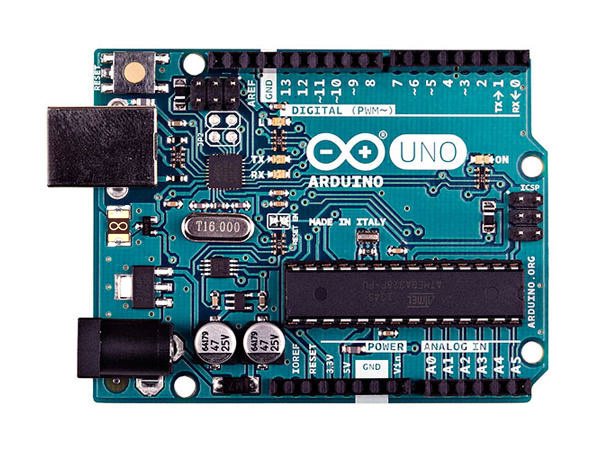
\includegraphics[width=7cm]{image/arduino_uno.jpg}
    }
  \caption{Microcontrôleur Arduino Uno}
\end{figure}

Arduino/Genuino Uno est un microcontrôleur  basé sur le soc ATmega328P. Il a 14 pins entrée/sortie pins (dont 6 qui peuvent être utilisés comme prise de courant 5v), 6 entrées analogiques, 16 MHz de fréquence, une connexion USB, une prise de courant, une tête ICSP et un bouton remise a zéro.\\

\subsubsection{Shield WiFi Arduino}

\begin{figure}[H]
  \centering
  \href{https://www.arduino.cc/en/Main/ArduinoWiFiShield}{
  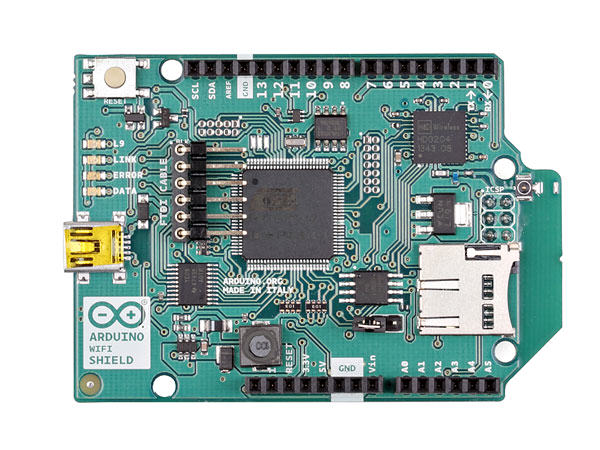
\includegraphics[width=7cm]{image/arduino_wifi.jpg}
  }
  \caption{Shield Wifi Arduino}
\end{figure}

L'Arduino WiFi Shield\footnote{"Bouclier" en anglais, c'est une carte conçue pour et ajouter des fonctionnes se poser sur l'Arduino} permet de relié l'Arduino à Internet sans fil.

\begin{itemize}
\item Nécessite un Arduino pour fonctionner.
\item Tension de service 5V (fournie par la carte Arduino). 
\item Arduino Due compatible.
\item Connexion via: réseaux 802.11b/g.
\item Types de cryptage: WEP et WPA2 personnels.
\item Connexion avec Arduino sur le port SPI.
\item Slot micro SD embarqué.
\item En-têtes ICSP.
\item Connexion FTDI pour le débogage en série du bouclier WiFi.
\item mini-USB pour la mise à jour du micrologiciel du bouclier WiFi.
\end{itemize}




\subsubsection{Shield bluetooth Arduino}

\begin{figure}[H]
  \centering
  \href{https://www.seeedstudio.com/Seeed-BLE-Shield-p-1859.html}{
  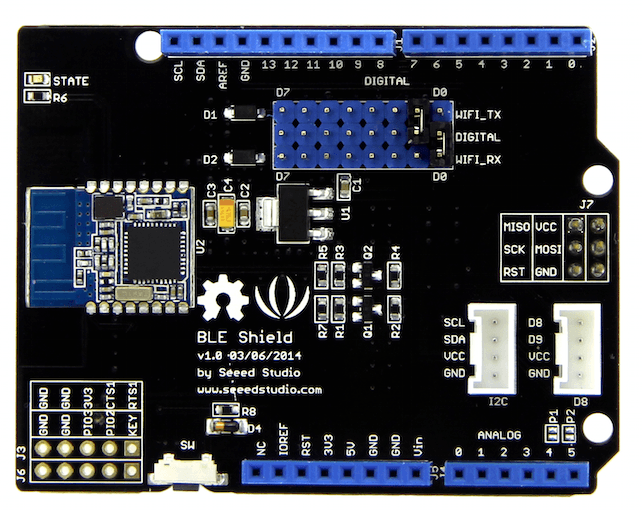
\includegraphics[width=7cm]{image/arduino_ble.png}
  }
  \caption{Shield Bluetooth Arduino}
\end{figure}

Le Bluetooth Shield intègre un module Serial Bluetooth. Il peut être facilement utilisé avec Arduino pour une communication série sans fil transparente. on peut  choisir deux broches d'Arduino D0 à D7 en tant que Ports Serial\footnote{ Transmission série} Serial pour communiquer avec Bluetooth Shield (D0 et D1 est Hardware Serial Port). La shield comporte également deux connecteurs \href{https://www.seeedstudio.com/Grove-Universal-4-pin-connector-p-789.html}{Grove}  (l'un est numérique, l'autre est analogique) pour installer des modules Grove.



\subsubsection{Capteurs de gaz MQ2, MQ6, MQ8}

\begin{figure}[H]
  \centering
  \href{http://playground.arduino.cc/Main/MQGasSensors}{
  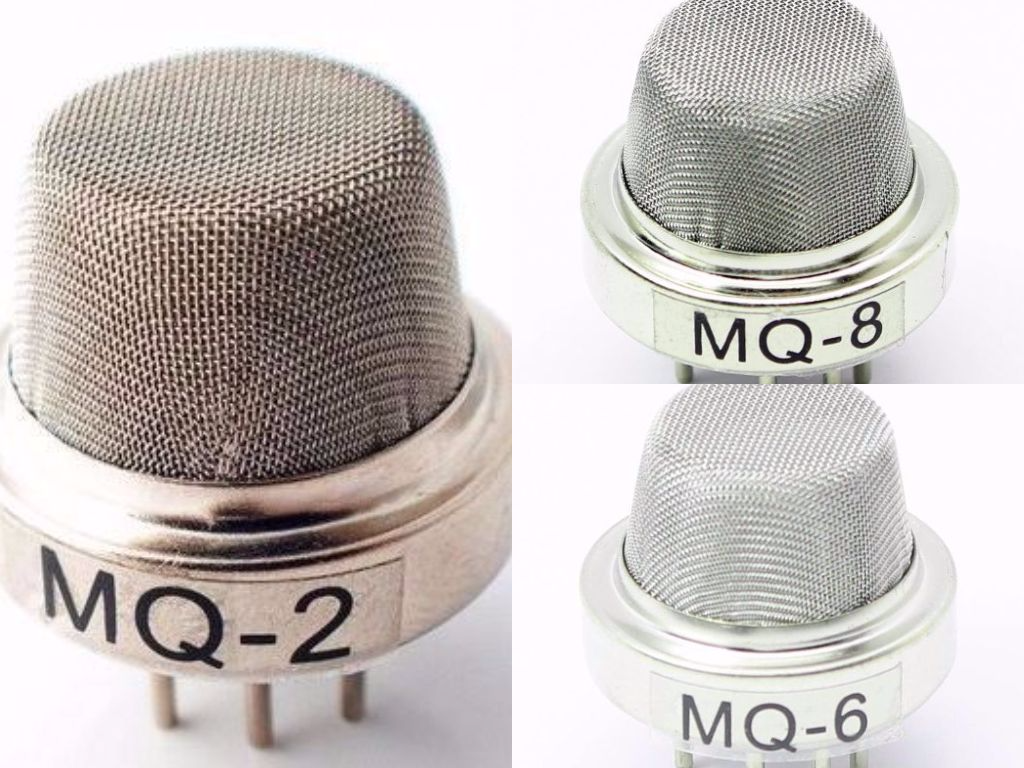
\includegraphics[width=7cm]{image/mq.png}
  }
  \caption{Capteurs de gaz MQ2,MQ6,MQ8}
\end{figure}

\begin{itemize}
\item Le capteur MQ2 peut être utilisé pour la détection de H2, LPG\footnote{Liquefied petroleum gas}, CH4, CO, Alcool, fumée ou Propane. 
\item Le capteur MQ6 peut être utilisé pour la détection de LPG ou CH4. 
\item Le capteur MQ8 peut être utilisé pour la détection de H2.

\end{itemize}


%sec%
\subsubsection{ESP8266}

\begin{figure}[H]
  \centering
  \href{https://fr.wikipedia.org/wiki/ESP8266}{
  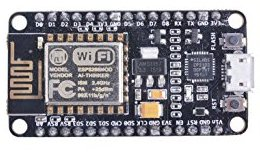
\includegraphics[width=7cm]{image/esp8266.png}
  }
  \caption{ESP8266-12E}
\end{figure}

L’ESP8266 est un circuit intégré à microcontrôleur avec connexion Wifi développé par le fabricant chinois \href{https://espressif.com/}{Espressif}.\\
Voici ses caractéristiques techniques:\\
\begin{itemize}

\item 32-bit RISC CPU: Tensilica Xtensa LX106, 80 MHz 64 KiB d’instructions RAM, 96 KiB de RAM de données.
\item QSPI flash externe - 512 KiB jusqu’à 4 MiB (support jusqu’à 16 MiB), IEEE 802.11 b/g/n Wifi.
\item TR switch intégré, balun\footnote{Un balun est un circuit électrique utilisé pour effectuer la liaison entre : une ligne de transmission symétrique (ligne bifilaire ou lignes imprimées parallèles) et une ligne de transmission asymétrique (câble coaxial ou ligne imprimée au-dessus d'un plan de masse)}, LNA, amplificateur de signal Wifi et compatibilité avec les réseaux WEP or WPA/WPA2, 16 GPIO pins ,SPI, I2C,I2S interfaces avec DMA (partage de pins avec GPIO).
\item UART dans les pins dédies , 10-bit ADC.
\end{itemize}

J’ai présenté en haut les matériels le plus importants pour la réalisation du projet, il y a toute la connectique derrière que je ne présenterai pas dans ce rapport.


\subsection{Logiciels}

\subsubsection{Arduino IDE}

\begin{figure}[H]
  \centering
  \href{https://www.arduino.cc/en/main/software}{
  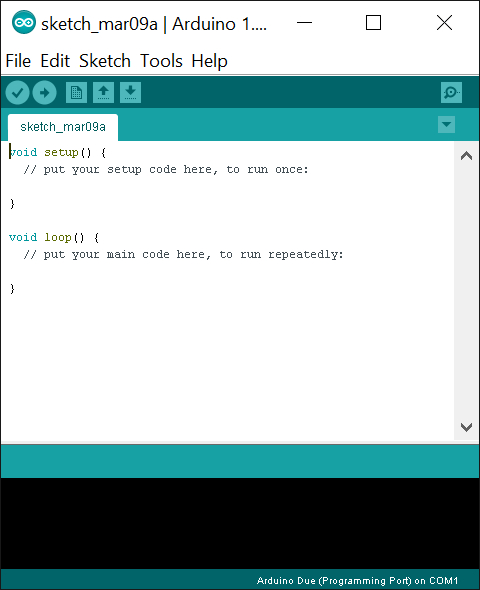
\includegraphics[width=8cm,height=8cm]{image/arduino_ide.png}
  }
  \caption{Arduino Web IDE}
\end{figure}
L'IDE est bon pour un début mais ensuite, je me suis rendu compte qu'il est pas assez puissant lors de la phase de débogage.
J'ai opté pour  la solution Arduino Cmake qui est parfaite pour les besoins de mon projet.

\subsubsection{Arduino CMake}

Arduino est une plate-forme de développement formidable, facile à utiliser. Il a tout ce dont un débutant devrait avoir besoin. L'IDE Arduino simplifie beaucoup de choses pour l'utilisateur standard, mais si vous êtes un programmeur professionnel, l'IDE peut paraître simpliste et restrictif.

Un inconvénient majeur de l'IDE d'Arduino est que je ne peux rien faire sans celui-ci, ce qui pour moi est une destruction totale. C'est pourquoi j'ai utilisé un système de construction alternatif pour Arduino.

\href{https://github.com/queezythegreat/arduino-cmake}{CMake} est un excellent système de construction multiplateforme qui fonctionne sur pratiquement n'importe quel système d'exploitation. Avec cela, on n'est pas contraint à un seul système de construction. CMake me permet de générer le système de construction qui correspond à mes besoins. Il peut générer tout type de système de construction, à partir de simples Makefiles, pour compléter des projets pour Eclipse, Visual Studio, XCode, etc.

Le système de construction Arduino CMake s'intègre étroitement au SDK Arduino qui doit être installé au préalable (Si l'IDE Arduino est installé sur la machine implique que le SDK est déjà installé sur votre système).

Pour pouvoir compiler sous Linux il faudra avoir les logiciel suivant sur la machine de développement  :

\begin{itemize}
\item gcc-avr - AVR GNU GCC compilateur 
\item binutils-avr - AVR outils binaire
\item avr-libc - AVR C librairie
\item avrdude - utiliser pour charger le firmware.
\end{itemize}


\subsubsection{Espruino IDE}

Espruino est un interpréteur JavaScript pour les microcontrôleurs. Il est conçu pour les appareils dotés d'un flash de 128kB et d'une RAM de 8kb.

\begin{figure}[H]
  \centering
  \href{https://www.espruino.com/}{
  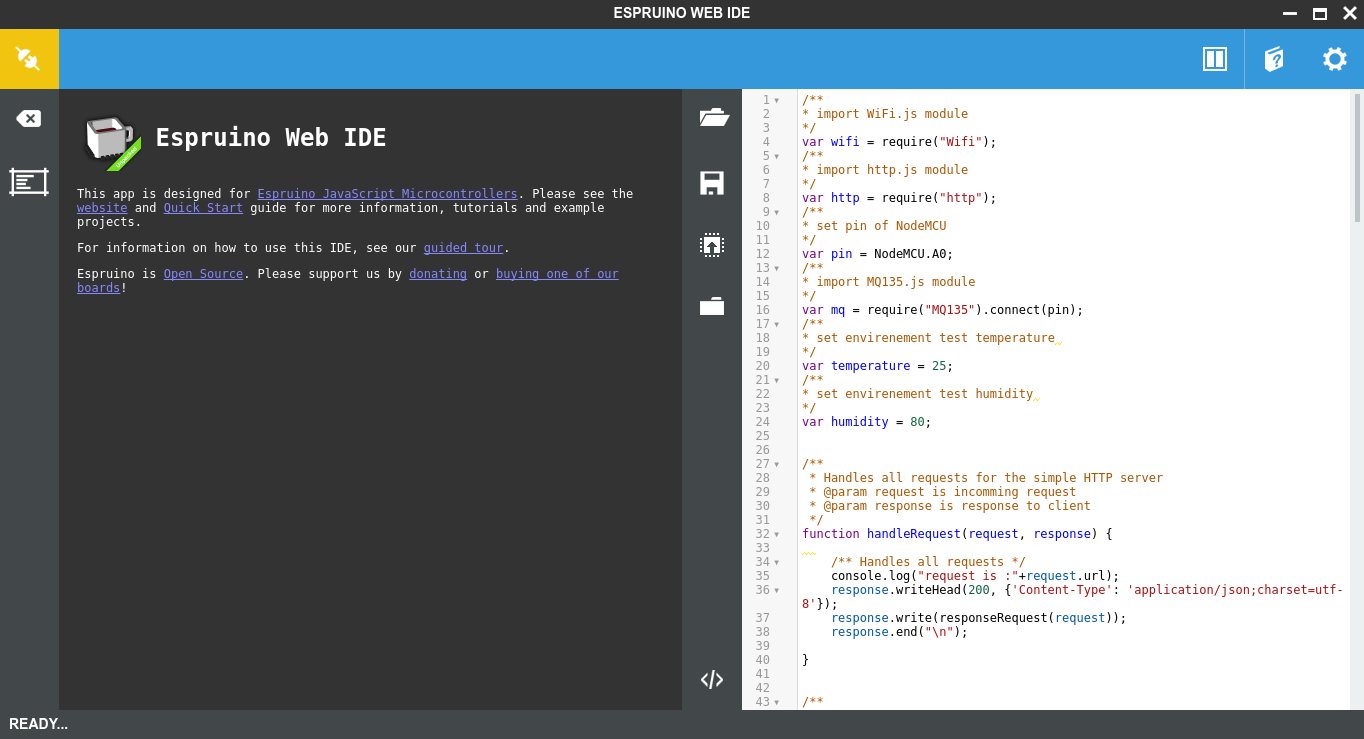
\includegraphics[width=15cm]{image/web00.png}
  }
  \caption{Espruino Web IDE}
\end{figure}

L'IDE peut être intégré au navigateur Chrome ou Chromium (version open source de chrome) sous la forme d'une extension qu'on peut installer du Chrome \href{https://chrome.google.com/webstore/detail/espruino-web-ide/bleoifhkdalbjfbobjackfdifdneehpo}{web store} ou à partir du dépôt \href{https://github.com/espruino/EspruinoWebIDE}{GitHub}  officiel.  

il est disponible également sous la forme d'un module \href{https://www.npmjs.com/package/espruino}{Node.js}  pour les puristes de la ligne de commande.

\begin{figure}[H]
  \centering
  \href{https://github.com/espruino/EspruinoTools}{
  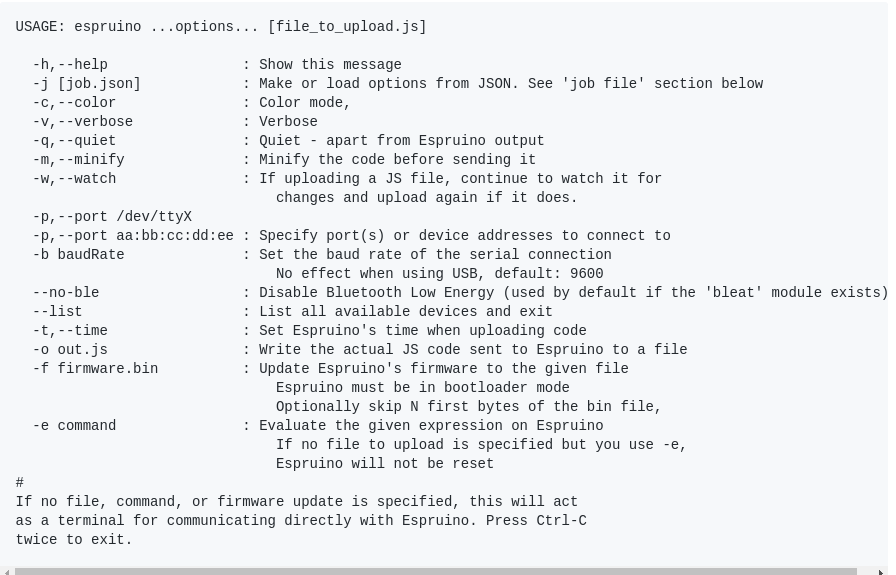
\includegraphics[width=15cm]{image/espruino_tools.png}
  }
  \caption{Espruino tools sous ligne de commande}
\end{figure}

\subsubsection{Esptools}
Esptools est un outil utilisé pour flasher différentes versions d’ESP, le chargement du micrologiciel ESPRUINO permet l'utilisation sur le ESP8266.\\
\begin{figure}[H]
  \centering
  \href{https://github.com/espressif/esptool}{
  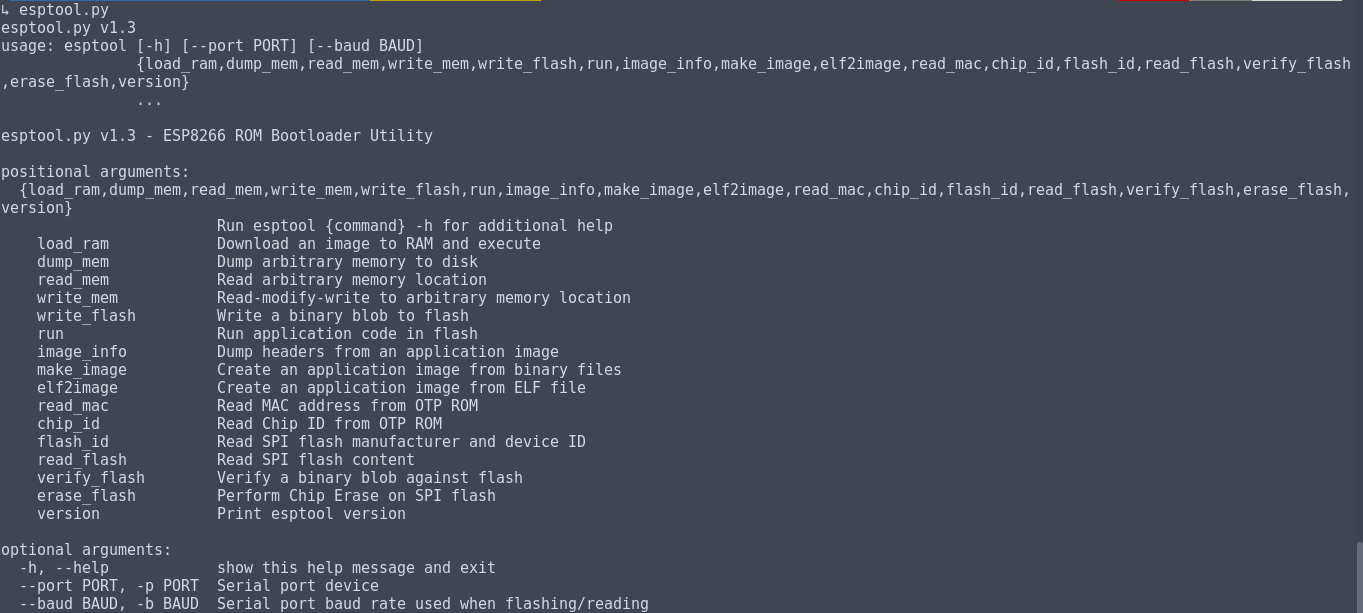
\includegraphics[width=15cm]{image/esptools.png}
  }
  \caption{Esptools}
\end{figure}
Il rend possible l'utilisation de JavaScript avec tous les microcontrôleurs supportés.\\
il est disponible également sous la forme d'un module \href{https://www.npmjs.com/package/esptool}{Node.js} pour les puristes de la ligne de commande.

\subsubsection{APISENSE}
La plate-forme APISENSE® permet de collecter une grande variété de données à partir des téléphones portables des usagers tout en garantissant le respect de leur vie privée. 
\begin{figure}[H]
  \centering
  \href{https://www.inria.fr/centre/lille/innovation/rii/rii-technologies-du-web/demos/apisense-r-accedez-a-une-foule-de-donnees-en-2-clics}{
  
\includegraphics[width=5cm]{image/apisense.png}
  }
  \caption{APISENSE}
\end{figure}

Utilisée dans de nombreux domaines, la plate-forme APISENSE® facilite la collecte, le stockage et le traitement des données renseignées par une foule d’usagers contributeurs. Basée sur les standards du web et déployée dans le Cloud, la plate-forme APISENSE® a notamment la capacité de traiter de gros volumes de données qui peuvent être restituées à différentes parties prenantes et sous différentes formes (OpenData, visualisations, etc.).




  %\include{partie/test}
  \newpage
\section{Implémentation}
Dans cette partie, j'expliquerai en détail le travail réalisé durant le semestre, la première phase de développement en langage C a pris la majeure partie du temps, pour la partie JavaScript,  c'était plutôt de l'adaptation de code.\\

Tout le code et la procédure de prise en main et d'installation sont disponibles sur le dépôt GitLab du projet et de l'archive jointe à ce rapport.\\


\subsection{Partie Arduino langage C}
\subsubsection{Structure du projet}
\begin{center}
\begin{tabular}{c c c}
\begin{minipage}{4cm}
 \begin{forest}
      for tree={
        font=\ttfamily,
        grow'=0,
        child anchor=west,
        parent anchor=south,
        anchor=west,
        calign=first,
        inner xsep=7pt,
        edge path={
          \noexpand\path [draw, \forestoption{edge}]
          (!u.south west) +(7.5pt,0) |- (.child anchor) pic {folder} \forestoption{edge label};
        },
        % style for your file node 
        file/.style={edge path={\noexpand\path [draw, \forestoption{edge}]
          (!u.south west) +(7.5pt,0) |- (.child anchor) \forestoption{edge label};},
          inner xsep=2pt,font=\small\ttfamily
                     },
        before typesetting nodes={
          if n=1
            {insert before={[,phantom]}}
            {}
        },
        fit=band,
        before computing xy={l=15pt},
      }  
    [oscar
      [build]
      [cmake
      	[ArduinoToolchain.cmake]
        [Platform[Arduino.cmake]]
      ]
      [CMakeLists.txt]
      [configure]
      [configure.bat]
      [doc[html]]
      [LICENCE]
      [README.md]
   	  ]
      \end{forest}
\end{minipage} 
& \makebox[3cm]{}
& \begin{minipage}{4cm}
       \begin{forest}
      for tree={
        font=\ttfamily,
        grow'=0,
        child anchor=west,
        parent anchor=south,
        anchor=west,
        calign=first,
        inner xsep=7pt,
        edge path={
          \noexpand\path [draw, \forestoption{edge}]
          (!u.south west) +(7.5pt,0) |- (.child anchor) pic {folder} \forestoption{edge label};
        },
        % style for your file node 
        file/.style={edge path={\noexpand\path [draw, \forestoption{edge}]
          (!u.south west) +(7.5pt,0) |- (.child anchor) \forestoption{edge label};},
          inner xsep=2pt,font=\small\ttfamily
                     },
        before typesetting nodes={
          if n=1
            {insert before={[,phantom]}}
            {}
        },
        fit=band,
        before computing xy={l=15pt},
      }  
      [oscar[src
      [AIRQUALIB[AIRQUALIB[AIRQUALIB.cpp,file][AIRQUALIB.h,file][CMakeLists.txt,file]]
      [examples[airqua\_ble[airqua\_ble.ino,file]][airqua\_eth[airqua\_eth.ino,file]]
      [airqua\_wifi[airqua\_wifi.ino,file]]]]
      [MQLIB[CMakeLists.txt][example[example.ino,file]][MQLIB[CMakeLists.txt,file][MQLIB.cpp,file][MQLIB.h,file]]]
      [V1AIRQUA[v1\_airqua\_ble[v1\_airquable.ino,file]][v1\_airqua\_eth[v1\_airqua\_eth.ino,file]]
      [v1\_airqua\_wifi[v1\_airqua\_wifi.ino,file]]]]]
      \end{forest}
\end{minipage}
\end{tabular}
\end{center}

\begin{verbatim}
--------------------------------------------------------------------------
Langage                      fichiers       espace    commentaire     code
--------------------------------------------------------------------------
Arduino Sketch                   7            273         457          792
C++                              2             43         110          149
C/C++ Header                     2             66         150           70
CMake                            5             38          46           60
--------------------------------------------------------------------------
TOTAL:                          16            420         763         1071
--------------------------------------------------------------------------

--------------------------------------------------------------------------
Fichiers                                       	 espace  commentaire  code
--------------------------------------------------------------------------
src/V1_AIRQUA/v1_airqua_ble/v1_airqua_ble.ino       51       100       180
src/V1_AIRQUA/v1_airqua_wifi/v1_airqua_wifi.ino     53       100       164
src/V1_AIRQUA/v1_airqua_eth/v1_airqua_eth.ino       51        69       135
src/AIRQUALIB/examples/airqua_ble/airqua_ble.ino    36        69       107
src/AIRQUALIB/examples/airqua_wifi/airqua_wifi.ino  39        68        90
src/AIRQUALIB/AIRQUALIB/AIRQUALIB.cpp               22        49        88
src/AIRQUALIB/examples/airqua_eth/airqua_eth.ino    34        38        62
src/MQLIB/MQLIB/MQLIB.cpp                           21        61        61
src/MQLIB/example/example.ino                        9        13        54
src/MQLIB/MQLIB/MQLIB.h                             47       111        50
src/AIRQUALIB/examples/CMakeLists.txt               13        14        20
src/AIRQUALIB/AIRQUALIB/AIRQUALIB.h                 19        39        20
src/V1_AIRQUA/CMakeLists.txt                        10        13        19
src/AIRQUALIB/AIRQUALIB/CMakeLists.txt               6         7         8
src/MQLIB/CMakeLists.txt                             5         6         7
src/MQLIB/MQLIB/CMakeLists.txt                       4         6         6
--------------------------------------------------------------------------
TOTAL:                                              420      763      1071
--------------------------------------------------------------------------

\end{verbatim}


\newpage
\subsubsection{MQLIB}
Dans cette première étape, j'ai commencé par la lecture des  fiches techniques des capteurs et de l'Arduino Uno r3.
Ensuite, j'ai continué la recherche sur les forums d'Arduino et des capteurs de gaz afin de récolter le maximum d'informations sur le matériels avant la phase de développement.\\

Le premier programme, appelé aussi croquis\footnote{Un programme écrit avec IDE pour Arduino s'appelle un croquis} Arduino, était très simple et consistait à lire une valeur analogique à partir des différents capteurs, afin de s'assurer de leurs bons fonctionnements.\\
\begin{lstlisting}
/* Pin sur lequel le capteur est connecter */
int sensorPin = A0;  

void setup() {
  /* UART reglages, baudrate = 9600bps.*/
  Serial.begin(9600); 
}

void loop() {
  /* Lecture et affichage de la valeur du capteur */
  Serial.print("Value of sensor is: "+analogRead(sensorPin);
  Serial.print("\");
}
\end{lstlisting}
Ensuite, j'ai implémenté un programme qui permet de lire des valeurs en PPM\footnote{Partie par million, fraction valant un millionième}, pour la liste des gaz supportés par les capteurs MQ (MQ2, MQ6, MQ8).\\
A la fin, j'ai intégré tout le code dans une libraire pour Arduino, qui facilite l'utilisation des capteurs avec un simple import.
\begin{lstlisting}
/* Declaration de la librairie MQLIB pour Arduino */
#ifndef MQLIB_H
#define MQLIB_H

#if ARDUINO >= 100
 #include "Arduino.h"
#else
 #include "WProgram.h"
#endif
...
#endif
}
\end{lstlisting}
j'ai ajouté un croquis qui permet de tester MQLIB et faciliter le travail des développeurs qui veulent l'utiliser ou l’améliorer.  
\begin{lstlisting}
void loop() {

  /* Q2 Sensor */
  Serial.print("MQ2 SENSOR");
  Serial.print("LPG:");
  Serial.print(air.displayGasValue(air.sensorA, GAS_LPG));
  Serial.print("ppm");
  Serial.print("    ");
  Serial.print("CO:");
  Serial.print(air.displayGasValue(air.sensorA, GAS_CO));
  Serial.print("ppm");
  Serial.print("    ");
  Serial.print("SMOKE:");
  Serial.print(air.displayGasValue(air.sensorA, GAS_SMOKE));
  Serial.print("ppm");
  Serial.print("\n");

  /* Q6 Sensor */
  Serial.print("MQ6 SENSOR");
  Serial.print("LPGQ6:");
  Serial.print(air.displayGasValue(air.sensorB, GAS_LPGQ6));
  Serial.print("ppm");
  Serial.print("        ");
  Serial.print("CH4::");
  Serial.print(air.displayGasValue(air.sensorB, GAS_CH4));
  Serial.print("ppm");
  Serial.print("\n");

  /* Q8 Sensor */
  Serial.print("MQ8 SENSOR");
  Serial.print("H2:");
  Serial.print(air.displayGasValue(air.sensorC, GAS_H2));
  Serial.print("ppm");
  Serial.print("\n");
  Serial.print("\n");
  delay(200);
}
\end{lstlisting}

\newpage
\subsubsection{AIRQUA}
J'ai implémenté un serveur web (REST) qui utilise MQLIB et peut être interrogé avec de simples requêtes GET, en fonction de la requête envoyée la réponse est renvoyée sous format JSON. Ensuite, j'ai intégré le serveur Web dans une librairie Arduino. 
\begin{lstlisting}
...
/** class declaration.*/
class AIRQUA {

...

/** 
* constructor3
* @param mq_pin1 - analog input channel you are going to use
* @param mq_pin2 - analog input channel you are going to use
* @param mq_pin3 - analog input channel you are going to use
*/
AIRQUA(uint8_t mq_pin1, uint8_t mq_pin2, uint8_t mq_pin3);

/**
 *  display current sensor value to client.
 *  @param sensorName is String argument which set sensor name.
 *  @param gasTypes is String argument which set sensor gas type.
 *  @param value is String argument which set sensor value.
 *  @return string sensor value
 */
    String sensorValue(String sensorName, String gasTypes, int value);


/**
 *  display sensor informations to client in Json format.
 *  @param sensorName is String argument which set sensor name.
 *  @param model is String argument which set sensor model.
 *  @param reference is String argument which set sensor reference.
 *  @param unite is String argument which set sensor unite.
 *  @param gasTypes is String argument which set sensor gas type (write it in
 * Json nested array format ex. "[\"LPG\",\"CO\",\"SMOKE\"]" ).
 *  @return string sensor informations
 */
    String sensorType(String sensorName, String model, String reference,String unite, String gasTypes);

/**
 *  display the response to the http request
 *  @param httpRequest is String argument which set http header content.
 *  @return response is String 
 */
    String responseRequest(String httpRequest);
};

#endif

\end{lstlisting}
\paragraph{Wifi:}
Cette version permet d’interroger AIRQUA en utilisant des requêtes GET via une connexion Wifi.

\begin{lstlisting}
...
void setup()
{
    /* Initialize serial and wait for port to open: */
    Serial.begin(9600);

    /* check for the presence of the shield: */
    if (WiFi.status() == WL_NO_SHIELD)
    {
        Serial.println("WiFi shield not present");

    }

    /* check firmware version */
    String fv = WiFi.firmwareVersion();
    if (fv != "1.1.0")
    {
        Serial.println("Please upgrade the firmware");
    }
      
    /* attempt to connect to Wifi network: */
    while (status != WL_CONNECTED && attemps <= 3)
    {
        Serial.print("Attempting to connect to SSID: ");
        Serial.println(ssid);
        /* Connect to WPA/WPA2 network. Change this */
        /* line if using open or WEP network: */
        status = WiFi.begin(ssid, pass);
        attemps++;
        /* wait 10 seconds for connection: */
        delay(10000);
    }
    
    /* start wifi server */
    server.begin();
    /* you're connected now, so print out the status: */
    printWifiStatus();
        
   ...
   
void printWifiStatus()
{
    /* print the SSID of the network you're attached to: */
    Serial.print("SSID: ");
    Serial.println(WiFi.SSID());

    /* print your WiFi shield's IP address: */
    IPAddress ip = WiFi.localIP();
    Serial.print("IP Address: ");
    Serial.println(ip);

    /* print the received signal strength: */
    long rssi = WiFi.RSSI();
    Serial.print("signal strength (RSSI):");
    Serial.print(rssi);
    Serial.println(" dBm");
}

\end{lstlisting}

\paragraph{Ethernet:}
C'est les mêmes fonctions que le serveur que Wifi sauf pour la partie connectique, il exploite un port Ethernet connecté à l'Arduino pour transférer les données.
\begin{lstlisting}
...
/** enter a MAC address and IP address for your controller below. */
byte mac[] = {
  0xDE, 0xAD, 0xBE, 0xEF, 0xFE, 0xED
};

/** the IP address will be dependent on your local network: */
IPAddress ip(192, 168, 1, 127);

/** 
 * initialize the Ethernet server library
 * with the IP address and port you want to use
 * (port 80 is default for HTTP):
 */
EthernetServer server(80);
...

\end{lstlisting}


\paragraph{Bluetooth:}
J'ai développé un programme qui permet une communication avec un périphérique doté de la technologie Bluetooth, pour mes essais j'ai utilisé un smartphone et un ordinateur.
Il permet les mêmes fonctionnalités que les deux versions précédentes, mais la partie communication est différente car l'utilisation du Bluetooth impose beaucoup de code en plus et davantage de restrictions pour le transfert des données.

\begin{lstlisting}
...
/** 
 * for Uno:
 * HM10 TX pin to Arduino Uno pin D6
 * HM10 RX pin to Arduino Uno pin D7
 * for Mega 2560: 
 * HM10 TX pin to Arduino Mega 2650 pin D10
 * HM10 RX pin to Arduino Mega 2560 pin D11
 */
SoftwareSerial ble(6,7);        

/** buffer to store response */
char buffer[BUFFER_LENGTH];   
...

/**
 *  Loop() is where the code that runms ovewr and over goes (your program).
 *  Listen to client requests and returns resposes.
 */
void loop() {
  
  if (ble.available()) {

    char request[200] = {0};
    int i = 0;
    while (ble.available()){
      char c = ble.read();
      request[i++] = c;
      delay(200); 
    }

    Serial.println(request);

    String response = airqua.responseRequest(request);
    /* display response for current client request */
    ble.println(response);

  } 
}

\end{lstlisting}

Les possibilités sont les suivantes:

- Valeur actuelle du capteur.
\begin{lstlisting}[language=bash]
curl --get http://192.168.0.21/sensors/co/value
{"name":"MQ2","gasTypes":"co","value":"0"}
\end{lstlisting}

- Type du capteur.
\begin{lstlisting}[language=bash]
sparow@debian:~$ curl --get http://192.168.0.21/sensors/h2/type
{"name":"Gas","model":"MQ8","reference":"MQ-8","unite":"PPM","gasTypes":["H2"]}
\end{lstlisting}

- Toutes les valeurs retournées par les capteurs.
\begin{lstlisting}[language=bash]
sparow@debian:~$ curl --get http://192.168.0.21/sensors/values
{"name":"MQ2","gasTypes":"co","value":"0"}
{"name":"MQ2","gasTypes":"smoke","value":"0"}
{"name":"MQ2","gasTypes":"lpg","value":"0"}
{"name":"MQ6","gasTypes":"lpg","value":"0"}
{"name":"MQ8","gasTypes":"h2","value":"0"}
{"name":"MQ6","gasTypes":"ch4","value":"0"}
\end{lstlisting}

- Tous les types disponibles.
\begin{lstlisting}[language=bash]
sparow@debian:~$ curl --get http://192.168.0.21/sensors/types
{"name":"Gas","model":"MQ2","reference":"MQ-2","unite":"PPM","gasTypes":["LPG","CO","SMOKE"]}
{"name":"Gas","model":"MQ6","reference":"MQ-6","unite":"PPM","gasTypes":["LPG","CH4"]}
{"name":"Gas","model":"MQ8","reference":"MQ-8","unite":"PPM","gasTypes":["H2"]}
\end{lstlisting}



\subsection{Partie ESP8266 JavaScript}


\subsubsection{Structure du projet}
\begin{forest}
      for tree={
        font=\ttfamily,
        grow'=0,
        child anchor=west,
        parent anchor=south,
        anchor=west,
        calign=first,
        inner xsep=7pt,
        edge path={
          \noexpand\path [draw, \forestoption{edge}]
          (!u.south west) +(7.5pt,0) |- (.child anchor) pic {folder} \forestoption{edge label};
        },
        % style for your file node 
        file/.style={edge path={\noexpand\path [draw, \forestoption{edge}]
          (!u.south west) +(7.5pt,0) |- (.child anchor) \forestoption{edge label};},
          inner xsep=2pt,font=\small\ttfamily
                     },
        before typesetting nodes={
          if n=1
            {insert before={[,phantom]}}
            {}
        },
        fit=band,
        before computing xy={l=15pt},
      }  
    [oscar-espruino
      [Installation.md,file]
      [README.md,file]
      [src
      [modules[MQ135.js,file][MQ135.min.js,file],[PrototypeMQLIB.js,file],[PrototypeMQLIB.min.js,file]]
      [projets[AirQua.js,file][examples[led\_blink.js,file]
      [wifi.js,file][wifi\_web\_server.js,file]]]
      ]
   	  ]
      \end{forest}
\begin{verbatim}
--------------------------------------------------------------------------
Langage                  fichiers       espace      commentaire       code
--------------------------------------------------------------------------
JavaScript                   8            100           244            274
--------------------------------------------------------------------------
TOTAL:                       8            100           244            274
--------------------------------------------------------------------------
\end{verbatim}
\newpage
\begin{verbatim}
--------------------------------------------------------------------------
Fichiers                                 espace      commentaire      code
--------------------------------------------------------------------------
src/projects/AirQua.js                     26             59            95
src/modules/PrototypeMQLIB.js              44            100            88
src/projects/examples/wifi_web_server.js    7             37            37
src/modules/MQ135.js                       20             39            36
src/projects/examples/wifi.js               2              7             9
src/projects/examples/led_blink.js          1              2             5
src/modules/MQ135.min.js                    0              0             3
src/modules/PrototypeMQLIB.min.js           0              0             1
--------------------------------------------------------------------------
TOTAL:                                    100            244           274
--------------------------------------------------------------------------

\end{verbatim}

\subsubsection{Prototype MQLIB}
J'ai commencé par une longue documentation sur le moteur JavaScript ESPRUINO et le microcontrôleur ESP8266.Ensuite, j'ai développé les exemples suivants:

- ledblink.js: permet de de faire clignoté la LED de l'ESP8266:

\begin{lstlisting}
var ledIsOn = false;
/ * 1000 milliseconds = 0.5 seconds */
var interval = 1000; 
setInterval(function(){
  /*D2 is the blue LED on the ESP8266 boards
  Assigns and flips the state on or off */
  digitalWrite(D2, ledIsOn = !ledIsOn);
}, interval);
\end{lstlisting}

- wifi.js: permet de se connecter à un réseau Wifi:


\begin{lstlisting}
var wifi = require("Wifi");

/**
 * Handles the connection for the wifi.connect call.
 * @param {Error} err
 */
function onConnect(err) {
    if(err) {
        console.log("An error has occured :( ", err.message);
    } else {
        console.log("Connected IP Adress : ", wifi.getIP().ip);
    }
}
wifi.connect("YourNetworkSSID", { password: "NetworkPassword" }, onConnect);
\end{lstlisting}

- wifiwebserver.js: c'est un serveur web qui affiche les réseaux Wifi disponibles autour:

\begin{lstlisting}
...

var http = require("http");
...

/**
 * Handles all requests for the simple HTTP server
 * 
 * @param {any} request - Incomming request
 * @param {any} response - Response to client
 */
function handleRequest(request, response) {
    //Handles all requests
    response.writeHead(200, {'Content-Type': 'text/html'});
    //Scans for accessible networks
    wifi.scan(function(networks){    
        response.end(generatePage("Networks", generateTableForAPs(networks)));
    });
}
...
\end{lstlisting}

Enfin, j'ai implémenté un prototype en JavaScript de MQLIB en m'inspirant d'un module existant et qui à était tester proprement sur ESPRUINO.

\begin{lstlisting}
exports.connect = function(mq_pin1, mq_pin2, mq_pin3) {
  return new MQLIB(mq_pin1, mq_pin2, mq_pin3);
}
/** 
* constructor3
* @param mq_pin1 - analog input channel you are going to use
* @param mq_pin2 - analog input channel you are going to use
* @param mq_pin3 - analog input channel you are going to use
*/
function MQLIB(mq_pin1, mq_pin2, mq_pin3)
{        
...
/**
* this gives the current gas value
* @param mq_pin - analog input channel
* @param gas_id - target gas type
* @return ppm of the target gas with the right sensor
*/
MQLIB.prototype.displayGasValue = function(mq_pin, gas_id)
{
    return (this.getGasPercentage(this.read(mq_pin) / this.tabR[mq_pin], gas_id));
}
\end{lstlisting}


\subsubsection{AIRQUA}
Suite à des restrictions matérielles liées ESP8266, qui contient un seul pin Analogique, j'ai implémenté un serveur avec un seul capteur (MQ135).
le serveur offre les mêmes fonctions que la version Wifi implémentée en langage C.

\begin{lstlisting}
...
/**
* import MQ135.js module
*/
var mq = require("MQ135").connect(pin);
...
/**
 *  display current sensor value to client.
 *  @param sensorName is String argument which set sensor name.
 *  @param is String argument which set sensor gas type.
 *  @param value is String argument which set sensor value.
 */
function sensorValue(sensorName, gasTypes , value)
{
    return ("{\"name\":\"" +sensorName+ "\",\"gasTypes\":\"" +gasTypes+ "\",\"value\":\"" +value+ "\"}\n");
 
}
/**
 *  display sensor informations to client in Json format.
 *  @param sensorName is String argument which set sensor name.
 *  @param model is String argument which set sensor model.
 *  @param reference is String argument which set sensor reference.
 *  @param unite is String argument which set sensor unite.
 *  @param gasTypes is String argument which set sensor gas type (write it in
 * Json nested array format ex. "[\"LPG\",\"CO\",\"SMOKE\"]" ).
 */
function sensorType(sensorName, model, reference,
    unite, gasTypes)
{
    return ("{\"name\":\"" +sensorName+ "\",\"model\":\"" +model+ "\",\"reference\":\"" +reference+ "\",\"unite\":\"" +unite+ "\",\"gasTypes\":" +gasTypes+ "}\n");
}
...
\end{lstlisting}

\newpage
\subsubsection{Tableau comparatif}
La liste des commandes et les résultats sont exactement les mêmes comparés à la version Arduino développée en langage C.

\begin{center}
\centering
\begin{tabular}{|p{7cm}|p{7cm}|}
\hline
Arduino C & Espruino JavaScript \\
\hline
\multicolumn{2}{|c|}{Avantages}\\
\hline
\hline
Gestion de la mémoire très efficace. & Rapidité d’exécution.\\
\hline
\hline
Faible consommation de ressources matériels & Code source court et compacte.\\
\hline
\hline
Support de plusieurs capteurs analogiques & Support de plusieurs capteurs numériques.\\
\hline
\hline
Support de la majorité des capteurs utilisés  & Processeur puissant et efficace \\
\hline
\hline
Environnement de développement complet  & Support natif de l'API RESTfull.   \\
\hline
\hline
\multicolumn{2}{|c|}{Inconvénients}\\
\hline
\hline
Non support natif de l'API RESTfull  & Consommation d'avantage de ressources matériels que Arduino\\
\hline
\hline
Problème de latence comparé à la version JavaScript  & Ajout obligatoire de Multiplexeur pour le support de plusieurs capteurs analogiques\\
\hline
\end{tabular}
\end{center}
  \section{Conclusion}

La solution que j'ai apportée correspond aux attentes dans la partie implémentée en langage C.\\

Je suis parti des connaissances acquises durant mon cursus universitaire. Par la suite, j'ai effectué des recherches qui m'ont permis de mettre en place les différentes parties du projet.\\

Les objectifs que je me suis fixés au début du PJI n'ont pas tous été réalisés. J'ai bien réussi la première partie, mais  pour la deuxième, j'ai eu trop de problèmes liés à la fois au matériel et logiciel. J'ai du changer le microcontrôleur, car Arduino Uno r3 n’était pas assez puissant pour supporter le moteur JavaScript et je l'es remplacé par le ESP8266 qui a ses avantages et ses inconvénients.\\

Ce PJI a été très intéressant et instructif. J'ai beaucoup appris sur le monde  de la recherche, ainsi que sur les connaissances qui seront utiles dans mon parcours.
Je suis très attiré par le monde de la recherche et parmi mes objectifs pour le PJI, je voulais me faire faire une idée plus précise de ce milieu. Cette expérience m'a permis de faire des rencontres avec des chercheurs dans le domaine qui m'intéresse. 
Grâce à ce PJI, j'ai pu travailler les connaissances que j'ai étudiées lors de mes cours du master.
C'est grâce à ce projet que j'ai eu une vraie idée sur le travail dans une équipe de recherche, et surtout à devenir autonome sur un projet concret.   
\newpage
  %\include{partie/annexe}
  
  % ne pas oublié de citer quelque chose pour que la biblio apparaisse
  \nocite{*}
  \bibliographystyle{alphadin}
  \bibliography{partie/biblio}
  
\end{document}
